\section{Unit testing}
We used a typical stub-driver approach to test the functionalities of main components of our applications. 
\newline
\newline
\hspace*{-1cm}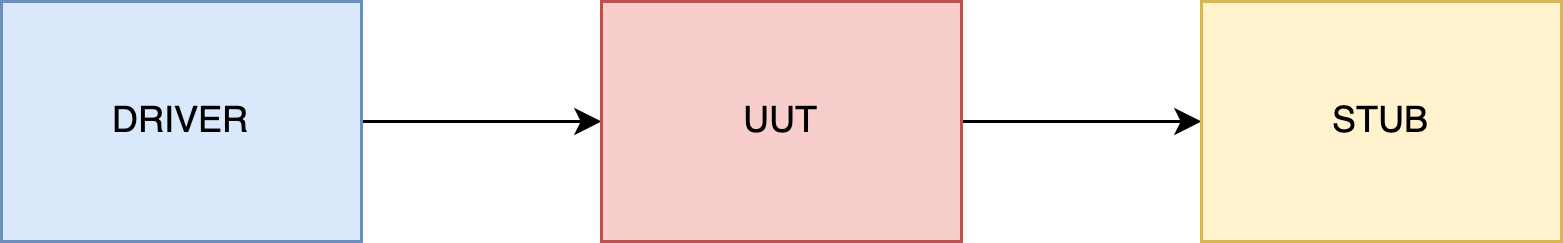
\includegraphics[width=14cm,keepaspectratio]{Images/testing/stub_driver.png}
\newpage
\noindent The tested components have been
\begin{itemize}
    \item[--] FirebaseAuthHelper
    \item[--] FirestoreHelper
    \item[--] ProductsProvider
    \item[--] ShoppingListProvider
\end{itemize}

\begin{wrapfigure}{r}{0.35\textwidth}
  \begin{center}
    \vspace*{-1cm}
\includegraphics[width=0.4\textwidth]{Images/testing/logo.png}
  \end{center}
\end{wrapfigure}
To mock their dependencies and create stubs, we used \textit{Mockito}, a powerful library that helps generating stubs.
In order for those components to be testable, we had to perform a refactoring to make them compliant to testable standard structure. One of the most important thing was to be able to inject dependencies via the constructor to create stubs for internal dependencies. We managed to accomplish this by dynamically resolve ad runtime the possibility to instantiate the object with some or all its dependencies mocked.
\newline
\newline
\begin{center}
    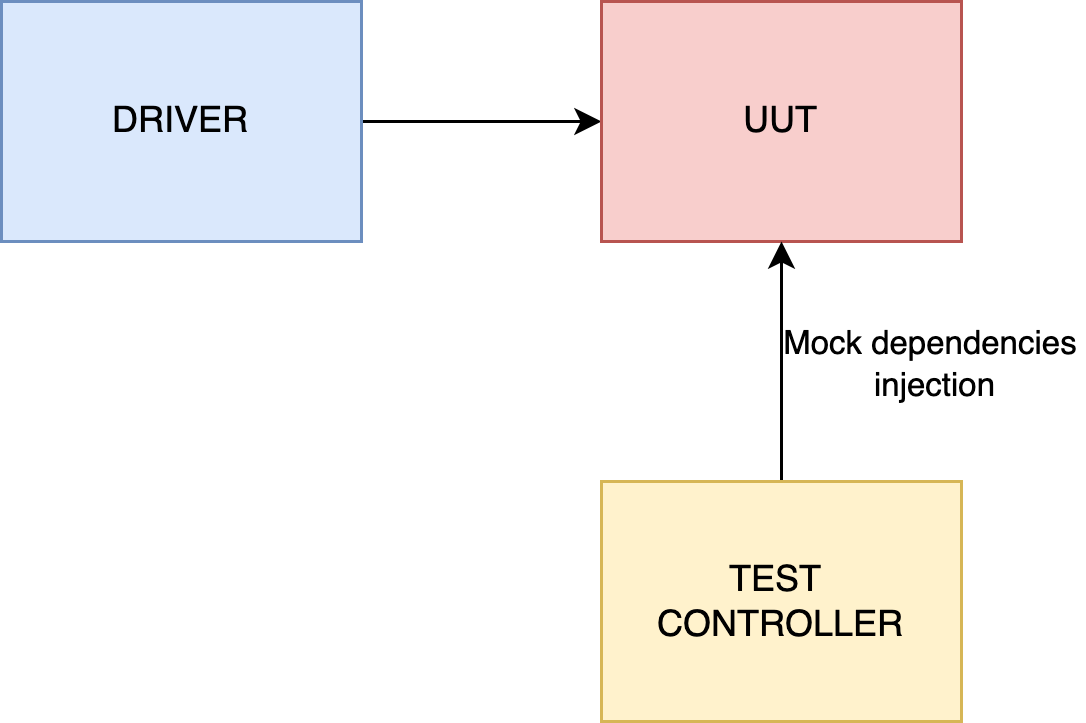
\includegraphics[width=8cm,keepaspectratio]{Images/testing/stub_driver_injection.png}
\end{center}

\noindent All of those components have been heavily tested in all of their use cases. We manage to obtain 60 tests (number also given from their complexity and dimension).
\newline
\newline
\noindent To perform assertions and evaluate tests we used the implemented flutter library called \textit{flutter\_test.dart}.

\newpage